\begin{frame}
  \frametitle{Legendre Polynomial Expansion of Inscattering Term}
  It is common to rewrite the inscattering (double-differential) cross section in terms of a Legendre polynomial expansion~\cite{Larsen2010}:
  \begin{equation}
    \label{eq:scattering-poly-expansion}
    \Sigma_s \left(\rvec,\ohat'\cdot \ohat,E'\rightarrow E\right) = \sum_{m=0}^{\infty}\frac{2m+1}{4\pi}P_m \left(\ohat' \cdot \ohat \right)\Sigma_{s,m}\left(\rvec, E'\rightarrow E\right)
  \end{equation}
  where $\Sigma_{s,m}\left(\rvec, E'\rightarrow E\right)$ are the \textit{Legendre moments}, computed with~\cite{TheoryManualOpenSn}:
  \begin{equation} \label{eq:legendre-moments}
    \Sigma_{s,m}\left(\rvec, E'\rightarrow E\right) = 2\pi \int_{-1}^{1}\Sigma_s \left(\rvec,\mu_0,E'\rightarrow E\right)P_m \left(\mu_0\right)\dd \mu_0
  \end{equation}
  where $\mu_0 \equiv \ohat' \cdot \ohat$.
  The moments are normally computed or available \textit{before} the simulation, \textit{not} computed on-the-fly.
  Note that \cref{eq:legendre-moments} is just an integral of the inscattering cross section over the unit sphere weighted by a Legendre polynomial.
\end{frame}

\begin{frame}
  \frametitle{Simplification of the \gls{bte}}
  Because the \glspl{arp} are stated to be \textit{non-multiplying}, \textit{time-independent}, and \textit{one-speed}, \cref{eq:general-bte} is immediately simplified to:
  \begin{multline}\label{eq:first-simplification-bte}
    \ohat \cdot \grad \psisimple + \Sigma_t \left(\rvec\right)\psisimple =\\=\int_{4\pi}\sum_{m=0}^{\infty}\frac{2m+1}{4\pi}P_m \left(\ohat' \cdot \ohat \right)\Sigma_{s,m}\left(\rvec\right)\psi \left(\rvec,\ohat'\right) \dd \ohat' + \frac{Q\left(\rvec\right)}{4\pi}
  \end{multline}
  Note that we have also substituted in \cref{eq:scattering-poly-expansion}.
\end{frame}

\begin{frame}
  \frametitle{Simplification of the \gls{bte}}
  The use of constant-value properties has a couple of immediate consequences, notably in the inscatter term.
  For a constant-value isotropic scattering cross section, \cref{eq:legendre-moments} is readily evaluated:
  \begin{equation}\label{eq:inscatter-xs-evaluated}
    \begin{split}
      \Sigma_{s,m}\left(\rvec\right) & = 2\pi \int_{-1}^{1}\Sigma_s \left(\rvec,\mu_0\right)P_m \left(\mu_0\right)\dd \mu_0       \\
                                     & =2\pi \int_{-1}^{1}\frac{\Sigma_s\left(\rvec\right)}{4\pi} P_m \left(\mu_0\right)\dd \mu_0 \\
                                     & =\frac{\Sigma_s\left(\rvec\right)}{2}\int_{-1}^{1} P_m \left(\mu_0\right)\dd \mu_0         \\
                                     & =\Sigma_s\left(\rvec\right) \delta_{0m}
    \end{split}
  \end{equation}
  where, in the last line, the orthogonality of Legendre polynomials is applied.

\end{frame}

\begin{frame}
  \frametitle{Simplification of the \gls{bte}}
  Substitution of \cref{eq:inscatter-xs-evaluated} into \cref{eq:first-simplification-bte} gives:
  \begin{equation}
    \ohat \cdot \grad \psisimple + \Sigma_t \left(\rvec\right)\psisimple =\frac{\Sigma_s\left(\rvec\right)}{4\pi}\int_{4\pi}\psi \left(\rvec,\ohat'\right) \dd \ohat' + \frac{Q\left(\rvec\right)}{4\pi}
  \end{equation}
  Or:
  \begin{equation} \label{eq:fully-simplified-bte-repeated}
    \ohat \cdot \grad \psisimple + \Sigma_t \left(\rvec\right)\psisimple =\frac{\Sigma_s\left(\rvec\right)}{4\pi}\phi\left(\rvec\right) + \frac{Q\left(\rvec\right)}{4\pi}
  \end{equation}
  where:
  \begin{equation}
    \label{eq:scalar-flux-repeated}
    \phi\left(\rvec\right)\equiv \int_{4\pi}\psi \left(\rvec,\ohat\right) \dd \ohat
  \end{equation}
  \Cref{eq:scalar-flux} is know as the \textit{angle-integrated} (or \textit{scalar}) \textit{flux}.
\end{frame}

\begin{frame}
  \frametitle{Error Plot}
  \begin{figure}
    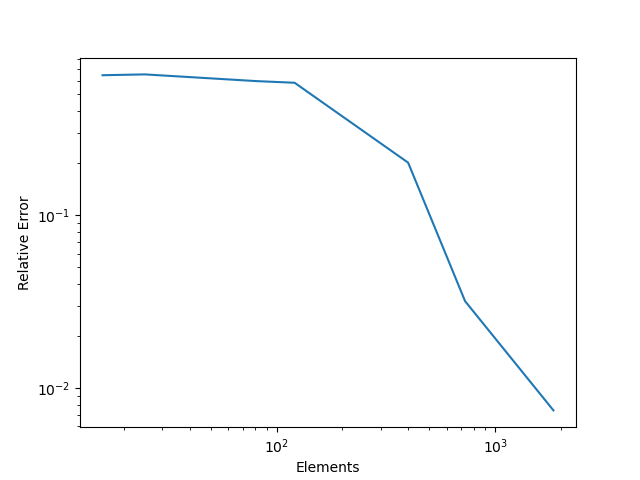
\includegraphics{figures/sphere/error.png}
    \caption{Error}
  \end{figure}
\end{frame}
